%% ---------- helpers for the result figures ----------
\newcommand{\uibox}[2]{{\setlength{\fboxsep}{0pt}\setlength{\fboxrule}{0.4pt}\fcolorbox{gray!55}{white}{\includegraphics[width=#1\linewidth]{#2}}}}
\newcommand{\resfig}[3]{\begin{center}{\renewcommand{\baselinestretch}{1}\selectfont #3}\end{center}\vspace{-8pt}\label{fig:#1}\figcap{#1}{#2}}
\pgfplotsset{resax/.style={width=0.93\linewidth,height=6.4cm,grid=major,grid style={gray!25},
  tick label style={font=\footnotesize},label style={font=\footnotesize},legend style={font=\footnotesize},
  every axis plot/.append style={line width=0.8pt}}}

\chap{6}{RESULTS AND DISCUSSIONS}{0pt}
\vspace{-8pt}
\sect{6.1}{DISCUSSIONS WITH DESCRIPTION AND SNAPSHOTS}
In the rapidly evolving field of genomic artificial intelligence, Evo2Serve represents a step towards making large genomic language models usable outside research notebooks. The web platform provides zero-shot, model-based assessments of genetic mutations by combining public genome and ClinVar data with Evo~2-7B served from a serverless H100 GPU. The primary outcomes of the project are a working sign-in, browse, analyse and compare workflow, a calibrated decision rule for \textit{BRCA1}, and a measured account of how the deployed pipeline relates to its calibration. Because the GPU, UCSC, NCBI and the account database are external services, the results below are drawn from the interface that can be shown without them and from the verification scripts of the project, which read the repository data and reproduce every figure and table without a GPU.

\hh{6.1.1 Secure Access: Sign-in and Account Creation Screen:}
\begin{itemize}
\item \textbf{Implementation:} The project began with the access layer of the web application. A single page, \texttt{/login}, switches between a ``Sign in'' and a ``Create account'' mode and posts the e-mail and password to the authentication routes.
\item \textbf{Functionality:} On success the server sets an HTTP-only cookie holding an HS256 session token valid for seven days and redirects to the main page. Wrong credentials and duplicate accounts return a message that the form displays under the fields.
\item \textbf{Public browsing and protected analysis:} The page states that browsing stays public. Assembly selection, chromosome browsing, gene search and sequence display need no account, whereas running the model requires one, so that the GPU cannot be used anonymously.
\item \textbf{Password handling:} Passwords are never stored. Only a bcrypt hash with ten rounds is written to the user collection, and the plain password is discarded after the check.
\item \textbf{Two-tier token check:} The same token is verified again by the Modal endpoint with the shared secret, so a request that bypasses the web tier still receives HTTP~401 from the GPU service.
\end{itemize}
\IfFileExists{images/ui_login.png}{%
\resfig{6.1.1}{Sign-in and Account Creation Screen}{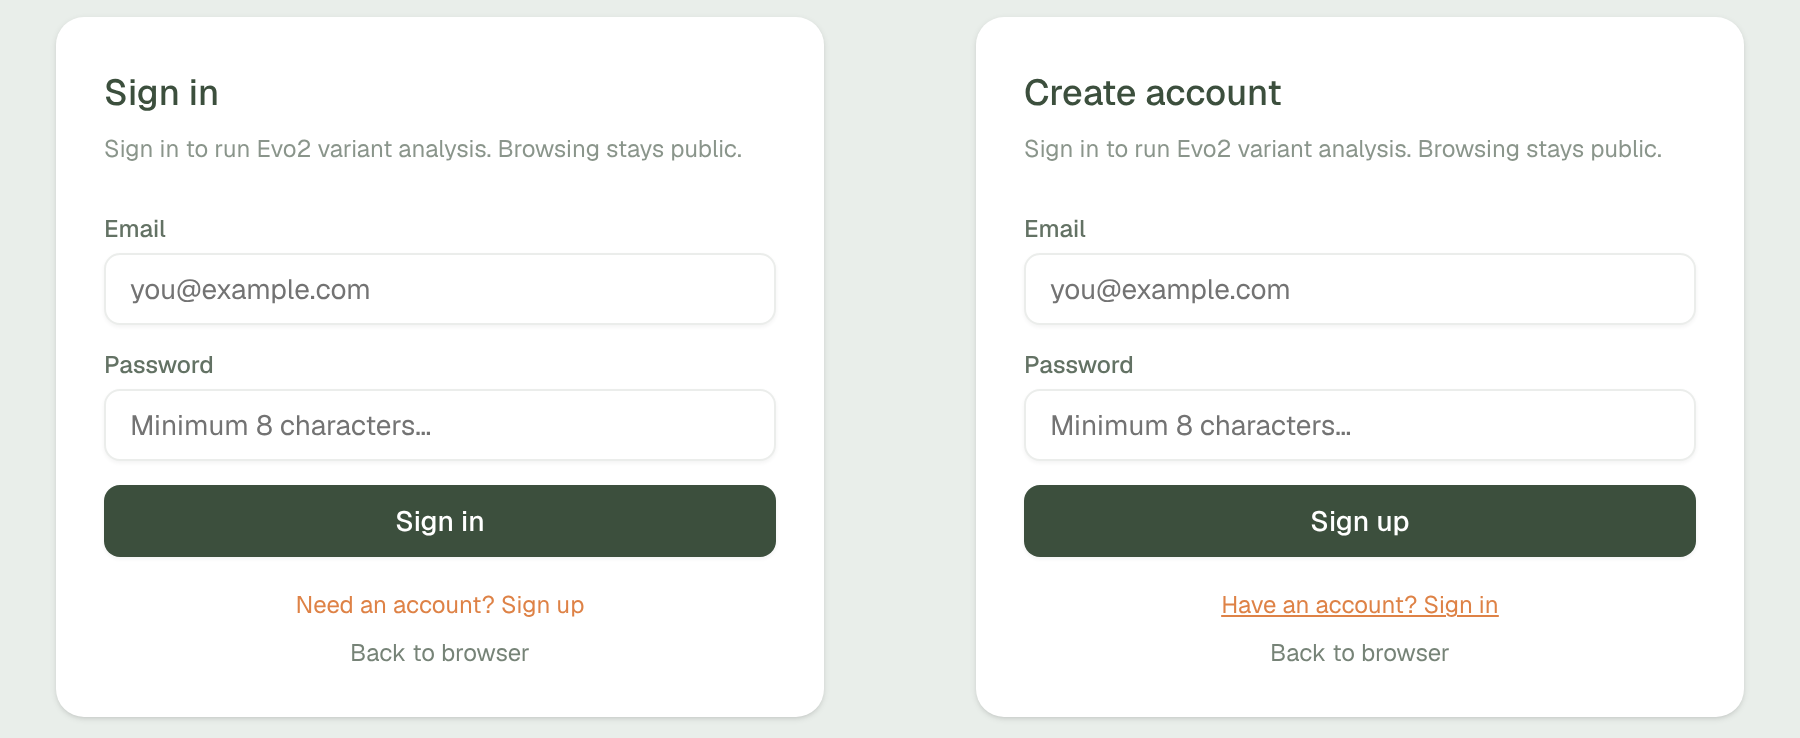
\includegraphics[width=0.78\linewidth]{images/ui_login.png}}}{%
\resfig{6.1.1}{Request Path of the Authenticated Analysis Call}{\diagSeq}}

\newpage
\hh{6.1.2 Calibration Data: Composition of the BRCA1 Assay and of the Calibration Set:}
\begin{itemize}
\item \textbf{Data Ingestion:} The saturation genome editing workbook of Findlay et al. was read directly from the Evo~2 repository. It holds 3,893 single-nucleotide variants of \textit{BRCA1}, each with a function score and a class.
\item \textbf{Reproduction of the Published Composition:} The workbook contains 2,821 functional (72.46\%), 249 intermediate (6.40\%) and 823 non-functional (21.14\%) variants, which reproduces the 72.5\%, 6.4\% and 21.1\% reported by the original study.
\item \textbf{Calibration Slice:} The deployed threshold was fitted on the first 500 rows only: 400 functional and 100 non-functional variants, a positive rate of 20.0\%, close to the 21.1\% of the whole assay.
\item \textbf{Data Integrity:} All 500 reference bases agree with the GRCh37 chromosome 17 sequence, and no window contains an ambiguous base.
\end{itemize}
\resfig{6.1.2}{Class Composition of the BRCA1 Assay and the Calibration Set}{%
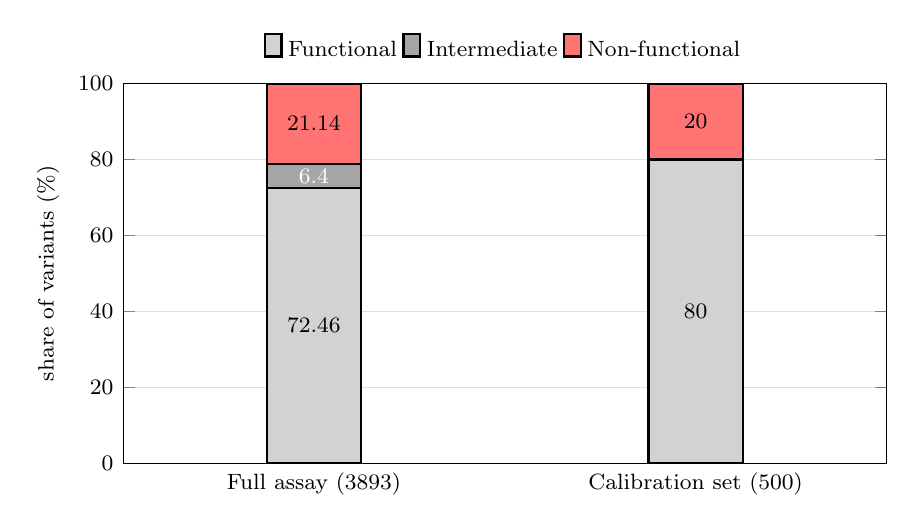
\begin{tikzpicture}
\begin{axis}[resax,ybar stacked,bar width=34pt,ymin=0,ymax=100,ylabel={share of variants (\%)},
  symbolic x coords={Full assay (3893),Calibration set (500)},xtick=data,enlarge x limits=0.5,
  nodes near coords,nodes near coords style={font=\footnotesize,text=black,anchor=center},
  legend style={at={(0.5,1.03)},anchor=south,legend columns=3,draw=none}]
\addplot[fill=gray!35] coordinates {(Full assay (3893),72.46) (Calibration set (500),80.0)};
\addplot[fill=gray!70,nodes near coords style={text=white,font=\footnotesize,anchor=center}] coordinates {(Full assay (3893),6.40) (Calibration set (500),0.0)};
\addplot[fill=red!55] coordinates {(Full assay (3893),21.14) (Calibration set (500),20.0)};
\legend{Functional,Intermediate,Non-functional}
\end{axis}
\end{tikzpicture}}

\newpage
\hh{6.1.3 Position Coverage of the Calibration Set:}
\begin{itemize}
\item \textbf{Genomic Span:} The 500 calibration variants lie between GRCh37 positions 41,267,755 and 41,276,135, a span of 8,380 bases, which is 10.69\% of the 78,413-base interval covered by the assay.
\item \textbf{Distinct Positions:} The slice touches 168 transcript positions and 41 amino-acid positions, against 1,326 and 326 in the whole assay.
\item \textbf{Reference Windows:} The 500 variants share only 168 distinct 8,192-base reference windows, because several substitutions occur at the same position.
\item \textbf{Consequence:} The histogram shows that the calibration set lies in two clusters at the end of the assayed interval. A threshold fitted on it describes the score distribution of that region of the gene, not of the whole gene and not of the genome.
\end{itemize}
\resfig{6.1.3}{Position Coverage of the Calibration Set}{%
\begin{tikzpicture}
\begin{axis}[resax,xlabel={position along the assayed interval (fraction)},ylabel={variants per bin},
  xmin=0,xmax=1,ymin=0,ymax=340,legend style={at={(0.5,1.03)},anchor=south,legend columns=2,draw=none}]
\addplot[ybar interval,fill=gray!50,draw=none,mark=none] coordinates {\coverageAll};
\addplot[ybar interval,fill=red!65,draw=none,mark=none] coordinates {\coverageSlice};
\legend{Full assay,Calibration set}
\end{axis}
\end{tikzpicture}}

\newpage
\hh{6.1.4 Reference Predictors: ROC Curves on the Calibration Set:}
\begin{itemize}
\item \textbf{Evaluation Design:} Five established predictors whose scores are stored in the workbook were evaluated on the same 500 rows, with loss of function as the positive class and the same Youden procedure that the calibration job uses.
\item \textbf{Strongest Predictor:} Align-GVGD separates the classes best (AUROC 0.878), followed by CADD (0.791) and phyloP (0.777).
\item \textbf{Weaker Predictors:} PolyPhen-2 (0.683) and SIFT (0.656) are clearly weaker, and population allele frequency (0.530) carries almost no signal, as expected for variants made by genome editing rather than drawn from a population.
\item \textbf{Missing Scores:} The missense-specific scores of Align-GVGD, PolyPhen-2 and SIFT exist for 268 of the 500 rows, because the other 232 variants are not missense changes.
\end{itemize}
\resfig{6.1.4}{ROC Curves of the Reference Predictors}{%
\begin{tikzpicture}
\begin{axis}[resax,xlabel={false positive rate},ylabel={true positive rate},xmin=0,xmax=1,ymin=0,ymax=1,
  legend style={at={(0.97,0.05)},anchor=south east,font=\footnotesize,fill=white,fill opacity=0.85,draw=gray!50}]
\addplot[dashed,gray,line width=0.5pt] coordinates {(0,0) (1,1)};
\addplot[very thick,red!75!black] coordinates {\rocaGVD};
\addplot[thick,blue!75!black] coordinates {\rocCADD};
\addplot[thick,green!50!black] coordinates {\rocphyloP};
\addplot[thick,orange!85!black] coordinates {\rocPolyPhen2};
\addplot[thick,teal!70!black] coordinates {\rocSIFT};
\legend{Random,Align-GVGD,CADD,phyloP,PolyPhen-2,SIFT}
\end{axis}
\end{tikzpicture}}

\newpage
\hh{6.1.5 AUROC with Bootstrap Confidence Intervals:}
\begin{itemize}
\item \textbf{Method:} Confidence intervals were obtained from 2,000 stratified bootstrap resamples with a fixed seed. The interval half-widths are about 0.03 to 0.07, so neighbouring predictors cannot be ranked with confidence on 500 variants.
\item \textbf{Evo~2-7B:} The zero-shot run of the calibration job reached an AUROC of approximately 0.73 on the same rows. This value is reported without an interval because the per-variant scores of that run were not archived.
\item \textbf{Comparison with the Whole Assay:} The published AUROC of CADD on all 3,893 variants is 0.8763, but only 0.791 on this slice. The same predictor moves by about 0.09 between the slice and the assay, so the slice is harder than the assay for every predictor.
\item \textbf{Interpretation:} A drop of Evo~2 from the published 0.9037 to about 0.73 is therefore consistent with the composition of the slice and not with a fault in the pipeline.
\end{itemize}
\resfig{6.1.5}{AUROC of the Predictors with 95\% Bootstrap Intervals}{%
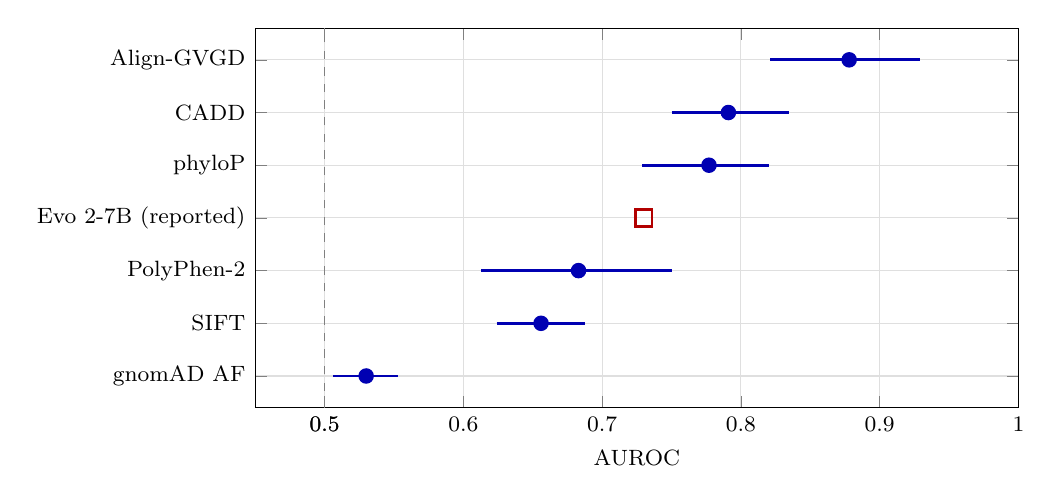
\begin{tikzpicture}
\begin{axis}[resax,xlabel={AUROC},xmin=0.45,xmax=1.0,ytick={1,2,3,4,5,6,7},
  yticklabels={gnomAD AF,SIFT,PolyPhen-2,Evo 2-7B (reported),phyloP,CADD,Align-GVGD},y dir=normal,ymin=0.4,ymax=7.6,
  extra x ticks={0.5},extra x tick style={grid=major,grid style={dashed,gray}}]
\addplot[only marks,mark=*,mark size=2.4pt,blue!70!black] coordinates {(0.530,1) (0.656,2) (0.683,3) (0.777,5) (0.791,6) (0.878,7)};
\addplot[only marks,mark=square,mark size=3pt,red!70!black,line width=1pt] coordinates {(0.73,4)};
\draw[line width=1pt,blue!70!black] (axis cs:0.506,1) -- (axis cs:0.553,1);
\draw[line width=1pt,blue!70!black] (axis cs:0.624,2) -- (axis cs:0.688,2);
\draw[line width=1pt,blue!70!black] (axis cs:0.613,3) -- (axis cs:0.750,3);
\draw[line width=1pt,blue!70!black] (axis cs:0.729,5) -- (axis cs:0.820,5);
\draw[line width=1pt,blue!70!black] (axis cs:0.750,6) -- (axis cs:0.835,6);
\draw[line width=1pt,blue!70!black] (axis cs:0.821,7) -- (axis cs:0.929,7);
\end{axis}
\end{tikzpicture}}

\newpage
\hh{6.1.6 Sensitivity and Specificity at the Youden Operating Point:}
\begin{itemize}
\item \textbf{Operating Points:} For each predictor the threshold that maximises sensitivity plus specificity minus one was chosen, the same rule that selects $\tau$ for Evo~2 in the calibration job.
\item \textbf{Trade-offs:} Align-GVGD has the best balance (sensitivity 0.762, specificity 0.917), CADD and phyloP favour sensitivity (0.90 and 0.88) at a specificity near 0.6, and SIFT calls almost every variant damaging (sensitivity 1.0, specificity 0.312).
\end{itemize}
\resfig{6.1.6}{Sensitivity and Specificity at the Youden Operating Point}{%
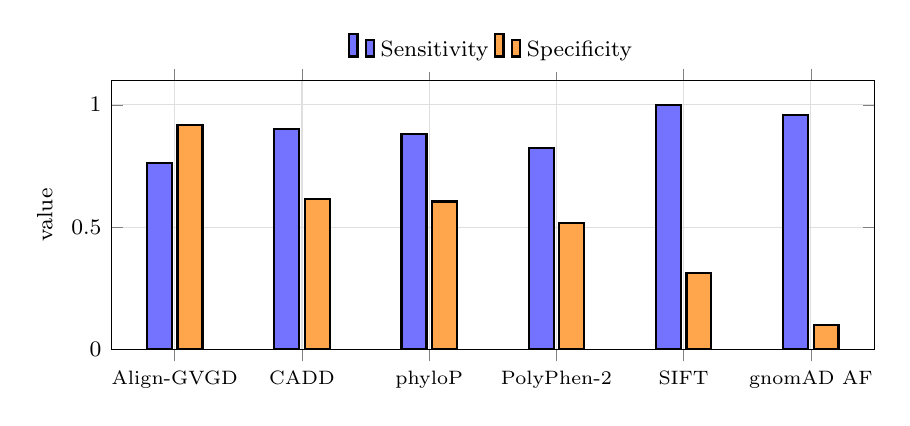
\begin{tikzpicture}
\begin{axis}[resax,ybar,height=5.0cm,bar width=9pt,ymin=0,ymax=1.1,ylabel={value},
  symbolic x coords={Align-GVGD,CADD,phyloP,PolyPhen-2,SIFT,gnomAD AF},xtick=data,
  x tick label style={font=\scriptsize},legend style={at={(0.5,1.03)},anchor=south,legend columns=2,draw=none}]
\addplot[fill=blue!55] coordinates {(Align-GVGD,0.762) (CADD,0.900) (phyloP,0.880) (PolyPhen-2,0.825) (SIFT,1.000) (gnomAD AF,0.960)};
\addplot[fill=orange!70] coordinates {(Align-GVGD,0.917) (CADD,0.615) (phyloP,0.605) (PolyPhen-2,0.517) (SIFT,0.312) (gnomAD AF,0.100)};
\legend{Sensitivity,Specificity}
\end{axis}
\end{tikzpicture}}
\vspace{-4pt}
\begin{center}
\footnotesize\renewcommand{\baselinestretch}{1}\selectfont
\label{tab:6.2}
Table 6.1: Reference Predictors on the 500-Variant BRCA1 Calibration Set\\[3pt]
\begin{tabular}{@{}lcccc@{}}
\toprule
Predictor & $n$ & AUROC & 95\% interval & Youden sens./spec. \\
\midrule
Align-GVGD & 268 & 0.878 & 0.821--0.929 & 0.762 / 0.917 \\
CADD & 500 & 0.791 & 0.750--0.835 & 0.900 / 0.615 \\
phyloP (mammalian) & 500 & 0.777 & 0.729--0.820 & 0.880 / 0.605 \\
PolyPhen-2 & 268 & 0.683 & 0.613--0.750 & 0.825 / 0.517 \\
SIFT & 268 & 0.656 & 0.624--0.688 & 1.000 / 0.312 \\
gnomAD allele frequency & 500 & 0.530 & 0.506--0.553 & 0.960 / 0.100 \\
\bottomrule
\end{tabular}
\end{center}

\newpage
\hh{6.1.7 Context Window: Deployed Endpoint versus Calibration Routine:}
\begin{itemize}
\item \textbf{Window Rule:} The calibration routine takes the interval of 4,096 bases on each side of the zero-based position, which is 8,192 bases with the variant at offset 4,096. The deployed endpoint takes one further base, giving 8,193 bases with the variant again at offset 4,096.
\item \textbf{Verification:} Over all 500 calibration positions the deployed window shares its first 8,192 bases with the calibration window and differs only by the final 3$'$ base; none of the 500 windows is identical, and no position is near a chromosome end.
\item \textbf{Consequence:} $\Delta$ is a difference of means over 8,193 positions in service and over 8,192 positions at calibration. The effect on the score is expected to be small, but its size cannot be measured without running the model, so it is listed as a limitation and as the first item of recalibration.
\end{itemize}
\resfig{6.1.7}{Context Window: Deployed Endpoint versus Calibration Routine}{%
\resizebox{0.93\linewidth}{!}{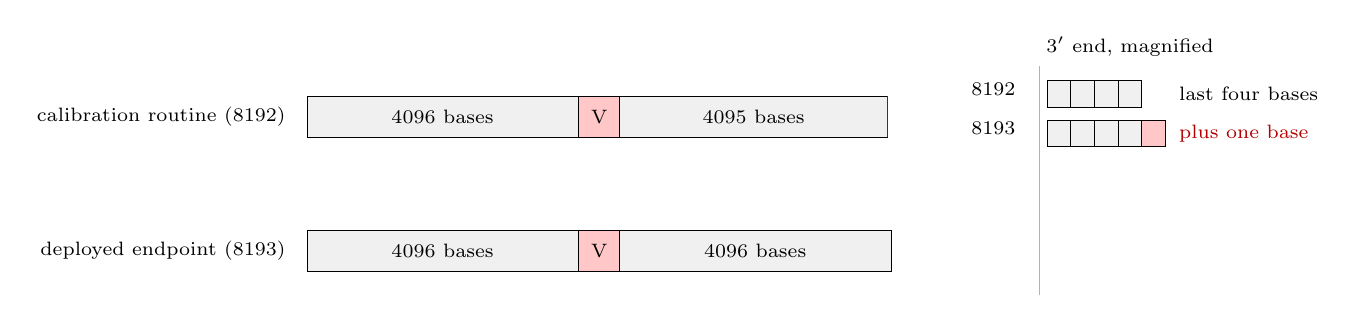
\begin{tikzpicture}[font=\scriptsize,
  seg/.style={rectangle,draw,minimum height=0.52cm,align=center,inner sep=1.5pt,line width=0.4pt},
  ctxs/.style={seg,fill=gray!12},vars/.style={seg,fill=red!22,minimum width=0.52cm},
  zc/.style={rectangle,draw,minimum width=0.30cm,minimum height=0.34cm,inner sep=0pt,line width=0.35pt},
  zx/.style={zc,fill=gray!12},zr/.style={zc,fill=red!22},note/.style={font=\scriptsize,anchor=west,inner sep=1pt}]
\draw[ctxs] (0,0.55) rectangle (3.45,1.07); \node at (1.72,0.81) {4096 bases};
\draw[vars] (3.45,0.55) rectangle (3.97,1.07); \node at (3.71,0.81) {V};
\draw[ctxs] (3.97,0.55) rectangle (7.37,1.07); \node at (5.67,0.81) {4095 bases};
\draw[line width=0.5pt,red!70!black] (7.37,0.55) -- (7.37,1.07);
\node[anchor=east] at (-0.15,0.81) {calibration routine (8192)};
\draw[ctxs] (0,-1.15) rectangle (3.45,-0.63); \node at (1.72,-0.89) {4096 bases};
\draw[vars] (3.45,-1.15) rectangle (3.97,-0.63); \node at (3.71,-0.89) {V};
\draw[ctxs] (3.97,-1.15) rectangle (7.42,-0.63); \node at (5.69,-0.89) {4096 bases};
\node[anchor=east] at (-0.15,-0.89) {deployed endpoint (8193)};
\draw[gray!60,line width=0.4pt] (9.30,-1.45) -- (9.30,1.45);
\node[align=center] at (10.45,1.70) {3$'$ end, magnified};
\node[anchor=east] at (9.12,1.16) {8192};
\foreach \i in {0,1,2,3} \node[zx] at (9.55+\i*0.30,1.10) {};
\node[anchor=east] at (9.12,0.66) {8193};
\foreach \i in {0,1,2,3} \node[zx] at (9.55+\i*0.30,0.60) {};
\node[zr] at (9.55+4*0.30,0.60) {};
\node[anchor=west] at (10.95,1.10) {last four bases};
\node[anchor=west,red!70!black] at (10.95,0.60) {plus one base};
\end{tikzpicture}}}

\newpage
\hh{6.1.8 Supported Mutation Types and Scored Sequence Lengths:}
\begin{itemize}
\item \textbf{Mutation Types:} The service applies four edit operations to the reference window: substitution, deletion, insertion and deletion--insertion, with deletions and insertions limited to 500 bases. An insertion is placed after the anchor base and a deletion--insertion replaces $n$ bases by the new bases.
\item \textbf{Length Check:} With a stand-in scorer in place of Evo~2, a substitution gives two sequences of 8,193 bases, a 3-base deletion gives 8,193 and 8,190 bases, and a 3-base insertion gives 8,193 and 8,196 bases, as the construction rules require.
\item \textbf{Mean-Score Effect:} When an edit changes the length, the reference and the mutated sequence are averaged over different numbers of positions, which is one reason why the indel predictions are flagged as provisional.
\end{itemize}
\resfig{6.1.8}{Supported Mutation Types and Scored Sequence Lengths}{%
\resizebox{0.72\linewidth}{!}{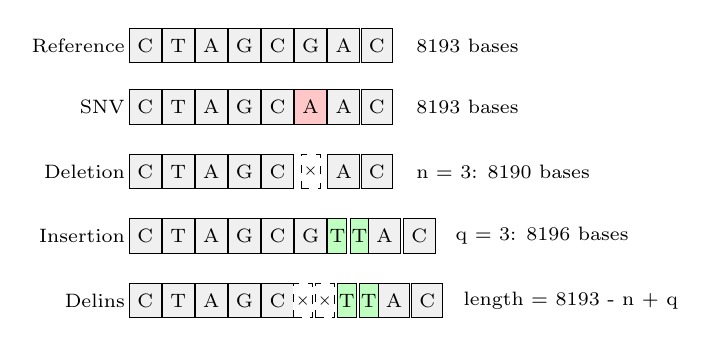
\begin{tikzpicture}[font=\scriptsize,
  cell/.style={rectangle,draw,minimum width=0.40cm,minimum height=0.44cm,align=center,inner sep=0pt,line width=0.35pt},
  ctx/.style={cell,fill=gray!12},altc/.style={cell,fill=red!22},
  nar/.style={rectangle,draw,minimum width=0.24cm,minimum height=0.44cm,align=center,inner sep=0pt,line width=0.35pt},
  insc/.style={nar,fill=green!25},gapc/.style={nar,dashed,fill=white},
  rowlbl/.style={font=\scriptsize,anchor=east,inner sep=1.5pt},note/.style={font=\scriptsize,anchor=west,inner sep=1pt}]
\node[rowlbl] at (-0.20,0) {Reference};
\foreach \b[count=\i from 0] in {C,T,A,G,C,G,A,C} \node[ctx] at (\i*0.42,0) {\b};
\node[note] at (3.4,0) {8193 bases};
\node[rowlbl] at (-0.20,-0.78) {SNV};
\foreach \b[count=\i from 0] in {C,T,A,G,C} \node[ctx] at (\i*0.42,-0.78) {\b};
\node[altc] at (2.10,-0.78) {A};
\foreach \b[count=\i from 6] in {A,C} \node[ctx] at (\i*0.42,-0.78) {\b};
\node[note] at (3.4,-0.78) {8193 bases};
\node[rowlbl] at (-0.20,-1.60) {Deletion};
\foreach \b[count=\i from 0] in {C,T,A,G,C} \node[ctx] at (\i*0.42,-1.60) {\b};
\node[gapc] at (2.10,-1.60) {\tiny$\times$};
\foreach \b[count=\i from 6] in {A,C} \node[ctx] at (\i*0.42,-1.60) {\b};
\node[note] at (3.4,-1.60) {n = 3: 8190 bases};
\node[rowlbl] at (-0.20,-2.42) {Insertion};
\foreach \b[count=\i from 0] in {C,T,A,G,C,G} \node[ctx] at (\i*0.42,-2.42) {\b};
\node[insc] at (2.44,-2.42) {T}; \node[insc] at (2.72,-2.42) {T};
\node[ctx] at (3.04,-2.42) {A}; \node[ctx] at (3.48,-2.42) {C};
\node[note] at (3.9,-2.42) {q = 3: 8196 bases};
\node[rowlbl] at (-0.20,-3.24) {Delins};
\foreach \b[count=\i from 0] in {C,T,A,G,C} \node[ctx] at (\i*0.42,-3.24) {\b};
\node[gapc] at (2.00,-3.24) {\tiny$\times$}; \node[gapc] at (2.28,-3.24) {\tiny$\times$};
\node[insc] at (2.56,-3.24) {T}; \node[insc] at (2.84,-3.24) {T};
\node[ctx] at (3.16,-3.24) {A}; \node[ctx] at (3.58,-3.24) {C};
\node[note] at (4.0,-3.24) {length = 8193 - n + q};
\end{tikzpicture}}}

\newpage
\hh{6.1.9 Decision Rule and Confidence Function:}
\begin{itemize}
\item \textbf{Decision Rule:} A variant is called ``Likely pathogenic'' when $\Delta<\tau=-9.18\times10^{-4}$ and ``Likely benign'' otherwise. The threshold is the Youden-optimal point of the ROC curve of $-\Delta$ on the calibration set.
\item \textbf{Confidence Function:} The confidence is the distance of $\Delta$ from $\tau$ divided by the spread of the predicted class ($\sigma_{LOF}=1.51\times10^{-3}$ or $\sigma_{FUNC}=9.02\times10^{-4}$), capped at one. It is a distance heuristic and not a calibrated probability.
\item \textbf{Null Edit:} A substitution that leaves the base unchanged gives $\Delta=0$ exactly, which is above $\tau$ and therefore ``Likely benign'' with confidence 1.0 (marked in the plot). This follows from the arithmetic of the function, and the planned reference-allele check would reject such a request.
\item \textbf{Stand-in Result:} For a substitution at a \textit{BRCA1} position the stand-in scorer returned $\Delta=-1.03\times10^{-4}$, the same order of magnitude as $\tau$.
\end{itemize}
\resfig{6.1.9}{Decision Rule and Confidence Function}{%
\begin{tikzpicture}
\begin{axis}[resax,xlabel={$\Delta$ score},ylabel={confidence},xmin=-0.004,xmax=0.002,ymin=0,ymax=1.08,
  scaled x ticks=false,xtick={-0.004,-0.003,-0.002,-0.001,0,0.001,0.002},
  xticklabel style={/pgf/number format/fixed,/pgf/number format/precision=3,font=\scriptsize},
  legend style={at={(0.02,0.35)},anchor=south west,fill=white,fill opacity=0.85,draw=gray!50}]
\addplot[thick,red!75!black,domain=-0.004:\confTau,samples=80] {min(1,abs(x-\confTau)/\confSigLOF)};
\addplot[thick,teal!70!black,domain=\confTau:0.002,samples=80] {min(1,abs(x-\confTau)/\confSigFUNC)};
\addplot[dashed,black,line width=0.5pt] coordinates {(\confTau,0) (\confTau,1.08)};
\addplot[only marks,mark=*,mark size=2.8pt,orange!85!black] coordinates {(0,1)};
\node[font=\scriptsize,anchor=south west] at (axis cs:0.0001,1.0) {null edit};
\node[font=\scriptsize,anchor=south] at (axis cs:\confTau,0.78) {$\tau$};
\legend{Likely pathogenic side,Likely benign side}
\end{axis}
\end{tikzpicture}}

\newpage
\hh{6.1.10 GRCh37 and GRCh38 Coordinates at the BRCA1 Locus:}
\begin{itemize}
\item \textbf{Assembly Offset:} The calibration data use GRCh37, but the service answers for GRCh38 by default. Aligning the two assemblies across \textit{BRCA1} with 681 conserved anchors gives a constant offset of 1,847,983 bases; all 680 consecutive anchor pairs are free of indels.
\item \textbf{Independent Confirmation:} The same offset appears in all 290 live ClinVar \textit{BRCA1} records that carry both a GRCh37 and a GRCh38 position, and agrees with the NCBI Gene model.
\item \textbf{Effect of a Wrong Assembly:} The same number read in the other assembly addresses a locus 1,847,983 bases away, that is, a different part of the genome. The example request shipped in the backend shows this: position 43,119,628 holds T in GRCh38, the same number holds C in GRCh37, and the 8,192-base windows around the two agree at only 25.2\% of positions, about what two unrelated sequences share by chance. After the correct conversion the reference base matches the assay for 500 of 500 calibration variants.
\item \textbf{Why It Matters:} The request carries no reference allele, so the service cannot detect the error and returns a confident answer either way. Sending the expected reference base and rejecting a mismatch is therefore the first planned improvement.
\end{itemize}
\resfig{6.1.10}{GRCh37 and GRCh38 Coordinates at the BRCA1 Locus}{%
\resizebox{0.8\linewidth}{!}{\begin{tikzpicture}[font=\scriptsize,
  ax/.style={-{Stealth[length=2.4mm]},line width=0.5pt},
  b/.style={rectangle,draw,rounded corners=2pt,minimum height=0.55cm,align=center,inner sep=2pt,line width=0.4pt}]
\node[b,fill=gray!12,minimum width=2.3cm] (g19) at (0,0) {GRCh37\\41,267,755};
\node[b,fill=gray!12,minimum width=2.3cm] (g38) at (5.9,0) {GRCh38\\43,115,738};
\node[b,fill=red!18,minimum width=2.9cm] (wrong) at (1.4,-2.3) {Same numeric coordinate\\43,115,738 in GRCh37};
\node[b,fill=green!18,minimum width=2.9cm] (right) at (4.5,-2.3) {Lifted coordinate\\43,115,738 in GRCh38};
\draw[ax] (g19.east) -- node[above,font=\scriptsize]{$+$1,847,983} (g38.west);
\draw[ax,red!70!black] (g19.south) -- (1.4,-1.35) -- (wrong.north);
\draw[ax,green!50!black] (g38.south) -- (4.5,-1.35) -- (right.north);
\node[font=\scriptsize,red!70!black,align=center] at (1.4,-3.35) {different base\\(example: C instead of T)};
\node[font=\scriptsize,green!50!black,align=center] at (4.5,-3.35) {$500/500$ reference bases\\correct};
\end{tikzpicture}}}

\newpage
\hh{6.1.11 Variant Types in the Live ClinVar Query:}
\begin{itemize}
\item \textbf{Query:} A ClinVar E-search for \textit{BRCA1} returned 300 records in the run reported here. Of these, 218 are single-nucleotide variants, 44 deletions, 15 duplications, 11 indels, 5 insertions and the remainder copy-number, haplotype or microsatellite records.
\item \textbf{Title Parsing:} The interface derives the variant type from the record title. In the 300 records, 280 are analysable and carry a usable numeric position; 42 are parsed as deletions, 20 as insertions and 13 as deletion--insertions.
\item \textbf{Coordinate Field:} The coordinate that the browser forwards to the endpoint is the \texttt{location\_sort} field, which equals the GRCh38 start in 293 of the 300 records and the GRCh37 start in none, even when hg19 is selected. The planned improvement is to read the position of the selected assembly.
\end{itemize}
\resfig{6.1.11}{Variant Types in the Live ClinVar BRCA1 Query}{%
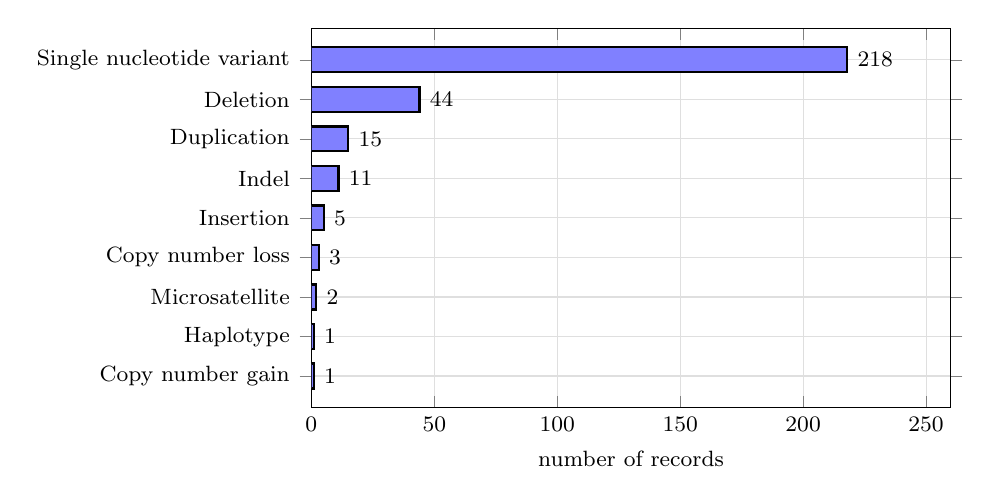
\begin{tikzpicture}
\begin{axis}[resax,width=0.8\linewidth,xbar,xlabel={number of records},xmin=0,xmax=260,y dir=reverse,
  symbolic y coords={Single nucleotide variant,Deletion,Duplication,Indel,Insertion,Copy number loss,Microsatellite,Haplotype,Copy number gain},
  ytick=data,y tick label style={font=\footnotesize},bar width=9pt,nodes near coords,nodes near coords style={font=\footnotesize}]
\addplot[fill=blue!50] coordinates {(218,Single nucleotide variant) (44,Deletion) (15,Duplication) (11,Indel) (5,Insertion) (3,Copy number loss) (2,Microsatellite) (1,Haplotype) (1,Copy number gain)};
\end{axis}
\end{tikzpicture}}

\newpage
\hh{6.1.12 Conformance of the Two Request Validators:}
\begin{itemize}
\item \textbf{Test Matrix:} A generated matrix of 55 request cases covers every discriminating field, both boundaries of every numeric constraint, the 500-base limit, whitespace handling and twelve malformed assembly and chromosome values. The expected verdict of each case comes from the request schema, not from either implementation.
\item \textbf{Outcome:} The Pydantic model of the GPU tier conforms on 43 cases and the Zod schema of the web tier on 47; both conform on 42. The two layers disagree on 6 cases, in all of which the web tier rejects the request before it reaches the GPU.
\item \textbf{Shared Defects:} Seven cases are handled wrongly by both layers. In six of them, assembly or chromosome values containing a semicolon, newline, slash or space are accepted although they should be rejected; the semicolon is the consequential one, because the backend places these values in a UCSC query string whose parameters are separated by semicolons. In the seventh, an alternate base with surrounding whitespace is rejected by both although the specification expects it to be accepted.
\end{itemize}
\resfig{6.1.12}{Conformance of the Two Request Validators}{%
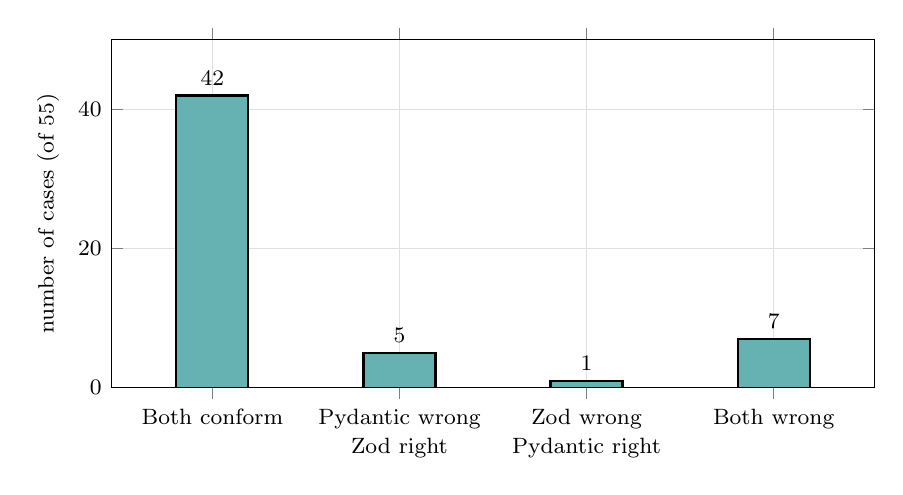
\begin{tikzpicture}
\begin{axis}[resax,ybar,height=6.0cm,bar width=26pt,ymin=0,ymax=50,ylabel={number of cases (of 55)},
  symbolic x coords={Both conform,Pydantic wrong\\Zod right,Zod wrong\\Pydantic right,Both wrong},xtick=data,
  x tick label style={font=\footnotesize,align=center},nodes near coords,nodes near coords style={font=\footnotesize},enlarge x limits=0.18]
\addplot[fill=teal!60] coordinates {(Both conform,42) (Pydantic wrong\\Zod right,5) (Zod wrong\\Pydantic right,1) (Both wrong,7)};
\end{axis}
\end{tikzpicture}}

\newpage
\hh{6.1.13 Class Balance of the Calibration Set along the Gene:}
\begin{itemize}
\item \textbf{Positive Rate:} The calibration set contains 100 non-functional rows, a positive rate of 20.0\%, close to the 21.1\% of the whole assay, but the rows are localised in one region of the gene (Section 6.1.3) and are not spread evenly within it.
\item \textbf{Imbalance within the Slice:} The first 250 rows contain 30 non-functional variants (12.0\%) and the last 250 contain 70 (28.0\%), a factor of 2.3. A threshold fitted on the whole slice therefore mixes two sub-populations whose class mix differs with position.
\item \textbf{Implication:} The threshold describes the score distribution of this part of \textit{BRCA1}. Recalibration on all 3,893 variants with a held-out split is the planned remedy.
\end{itemize}
\resfig{6.1.13}{Calibration Set Class Balance along the Gene}{%
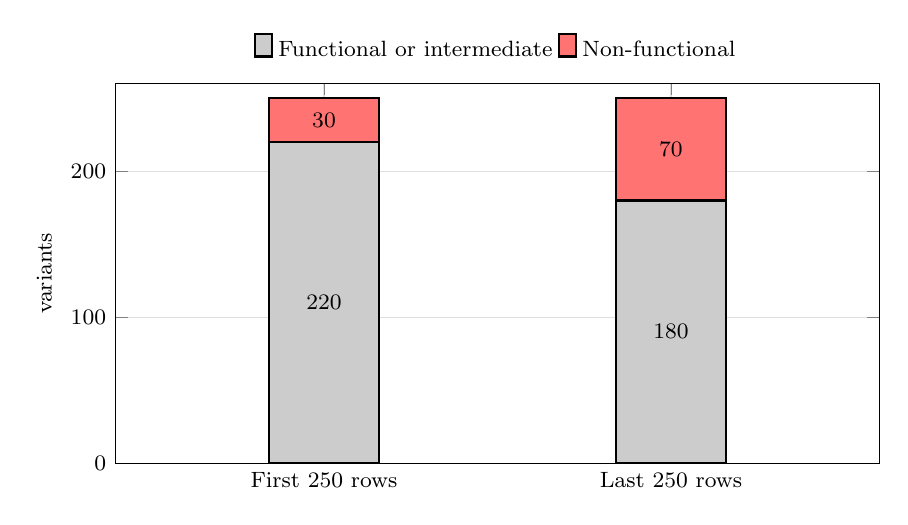
\begin{tikzpicture}
\begin{axis}[resax,ybar stacked,bar width=40pt,ymin=0,ymax=260,ylabel={variants},
  symbolic x coords={First 250 rows,Last 250 rows},xtick=data,enlarge x limits=0.6,
  nodes near coords,nodes near coords style={font=\footnotesize,anchor=center},
  legend style={at={(0.5,1.03)},anchor=south,legend columns=2,draw=none}]
\addplot[fill=gray!40] coordinates {(First 250 rows,220) (Last 250 rows,180)};
\addplot[fill=red!55] coordinates {(First 250 rows,30) (Last 250 rows,70)};
\legend{Functional or intermediate,Non-functional}
\end{axis}
\end{tikzpicture}}

\newpage
\hh{6.1.14 GPU Forward Passes per Request and per Calibration Run:}
\begin{itemize}
\item \textbf{Per Request:} The endpoint scores the reference window and the mutated window on every request, two forward passes over about 8,200 bases, and performs no caching across requests.
\item \textbf{Calibration Job:} The offline routine de-duplicates the reference windows. For 500 variants it scores 168 unique references and 500 mutated windows, 668 passes instead of the 1,000 of the naive count, which is 33.2\% fewer.
\item \textbf{Improvement:} The window is a function of the coordinate only, so the reference score of a window could be cached across requests, which could roughly halve the forward passes needed for repeated queries on the same window.
\item \textbf{Not Measured:} Latency and throughput were not measured. They depend on the deployment, the cold-start time of the container and the model, which are outside the scope of the verification environment.
\end{itemize}
\resfig{6.1.14}{GPU Forward Passes per Request and per Calibration Run}{%
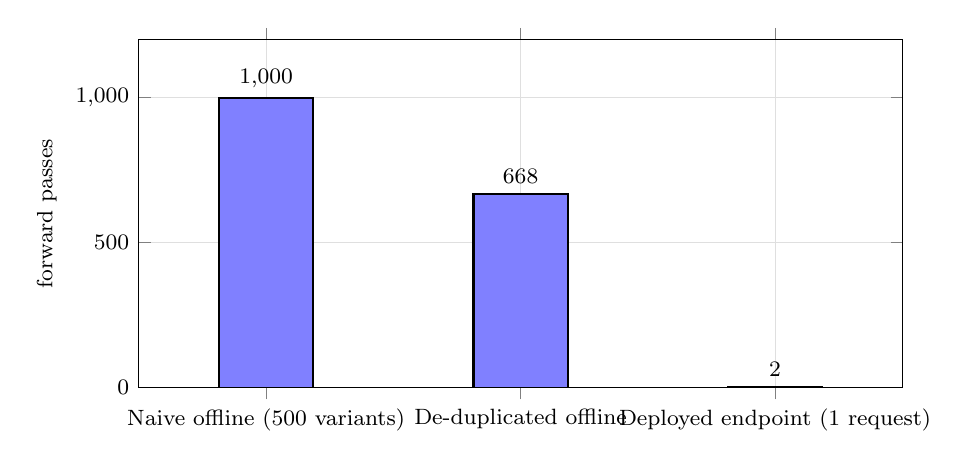
\begin{tikzpicture}
\begin{axis}[resax,ybar,height=6.0cm,bar width=34pt,ymin=0,ymax=1200,ylabel={forward passes},
  symbolic x coords={Naive offline (500 variants),De-duplicated offline,Deployed endpoint (1 request)},xtick=data,
  x tick label style={font=\footnotesize,align=center},nodes near coords,nodes near coords style={font=\footnotesize},enlarge x limits=0.25]
\addplot[fill=blue!50] coordinates {(Naive offline (500 variants),1000) (De-duplicated offline,668) (Deployed endpoint (1 request),2)};
\end{axis}
\end{tikzpicture}}

\newpage
\hh{6.1.15 Genome Browser: Assembly Selection, Gene Search and Chromosome Browsing:}
\begin{itemize}
\item \textbf{Implementation:} After sign-in the main page opens on the assembly selector, which is filled from the UCSC genome list and shows the human assemblies, with hg38 (GRCh38) active by default. Below it a Browse card offers two tabs.
\item \textbf{Gene Search:} The search box queries the NLM gene service and lists matching genes with their name, cytogenetic location and chromosome. A search for ``BRCA1 breast'' returns \textit{BRCA1} on 17q21.31 and \textit{BRCA2} on 13q13.1 (Figure~6.1.15).
\item \textbf{Chromosome Browsing:} The second tab lists chromosomes 1 to 22, M, X and Y of the selected assembly as buttons; choosing one lists the genes and regulatory elements found on it (Figure~6.1.16).
\item \textbf{Public Access:} Both tabs work without an account, because they only read public services.
\end{itemize}
\resfig{6.1.15}{Gene Search Results for BRCA1}{\uibox{0.9}{images/ui_search.png}}
\resfig{6.1.16}{Chromosome Browser for the hg38 Assembly (chr17 Selected)}{\uibox{0.9}{images/ui_browse.png}}

\newpage
\hh{6.1.17 Variant Entry and Known ClinVar Variants:}
\begin{itemize}
\item \textbf{Variant Entry:} Once a gene is chosen, the Variant Analysis card lets the user pick one of four mutation types: substitution, deletion, insertion or deletion--insertion. The fields change with the type; a substitution needs a position and an alternative base (Figure~6.1.17), a deletion a start position and a length, and the interface shows which reference base will be removed (Figure~6.1.18).
\item \textbf{Known Variants:} The Known Variants card lists the ClinVar records of the gene with their HGVS name, location, variant type and clinical significance, colour-coded as pathogenic, likely benign or uncertain significance (Figure~6.1.19).
\item \textbf{Analyse with Evo2:} A button next to each analysable record sends its coordinate to the model service. Duplications are listed without a button, since the service does not score them. The prediction panel is not shown, because it needs the GPU endpoint, which was not connected when these snapshots were taken.
\end{itemize}
\resfig{6.1.17}{Variant Entry Form: Substitution Mode}{\uibox{0.4}{images/ui_variant_snv.png}}
\resfig{6.1.18}{Variant Entry Form: Deletion Mode}{\uibox{0.4}{images/ui_variant_del.png}}
\resfig{6.1.19}{Known BRCA1 Variants from ClinVar}{\uibox{0.64}{images/ui_known.png}}

\newpage
\hh{6.1.20 Gene Sequence Viewer and Gene Information:}
\begin{itemize}
\item \textbf{Sequence Viewer:} The selected gene region is read from UCSC and drawn in rows of 200 bases with the coordinate of the first base, using one colour for each base: A red, T blue, G green and C orange. Two sliders and two number fields choose the window, which is limited to 10,000 bases, and a Load sequence button fetches it (Figure~6.1.20).
\item \textbf{Gene Information:} The Gene Information card shows the symbol, cytogenetic location, chromosome, genomic position and length of the gene, the Gene ID with a link to NCBI, the organism and the RefSeq summary (Figure~6.1.21).
\end{itemize}
\resfig{6.1.20}{Gene Sequence Viewer with Window Selection}{\uibox{0.85}{images/ui_sequence.png}}
\resfig{6.1.21}{Gene Information Card for BRCA1}{\uibox{0.85}{images/ui_geneinfo.png}}

\newpage
\label{tab:6.1}
Table 6.2: Test Results and Observations

\vspace{4pt}
\begingroup\fontsize{11}{13}\selectfont\renewcommand{\baselinestretch}{1.08}\selectfont
\renewcommand{\arraystretch}{1.45}
\noindent\begin{tabular}{|p{100pt}|p{112pt}|p{250pt}|}
\hline
Test Type & Result & Observations \\
\hline
Calibration data check & 3,893 of 3,893 rows read; 500 of 500 reference bases match & Composition 2,821 / 249 / 823 reproduces the published 72.5\% / 6.4\% / 21.1\%. \\
\hline
Window contract & 500 of 500 windows differ by one 3$'$ base & Deployed 8,193 bases against 8,192 at calibration; variant offset 4,096 in both. \\
\hline
Genome assembly & Lifted coordinate: 500 of 500 reference bases match; shipped example, same number: C instead of T & Constant offset of 1,847,983 bases, confirmed on 290 live ClinVar records. \\
\hline
Request validation, GPU tier (Pydantic) & 43 of 55 cases (78.2\%) & Accepts position zero, a negative position and empty genome or chromosome; accepts separator characters; rejects a whitespace-padded alternate base. \\
\hline
Request validation, web tier (Zod) & 47 of 55 cases (85.5\%) & Rejects the position and empty-field cases; accepts separator characters in assembly and chromosome; rejects a lowercase alternate base the specification accepts. \\
\hline
Scoring contract (stand-in scorer) & Lengths 8,193 / 8,190 (deletion) and 8,193 / 8,196 (insertion) & Mutation functions behave as specified; a null substitution yields $\Delta=0$ and confidence 1.0. \\
\hline
Live ClinVar integration & 300 records; 280 analysable & Coordinate forwarded is the GRCh38 start in 293 records and the GRCh37 start in none. \\
\hline
\end{tabular}
\endgroup

\vspace{8pt}
The verification confirmed that the data, the mutation functions and the live ClinVar integration behave as designed, and it located specific places where the deployed pipeline differs from the conditions of its calibration. The calibration data reproduce the published composition of the assay, all 500 reference bases agree with the reference sequence, and the mutation functions produce sequences of the expected length for every variant type.

The same evaluation identified eight improvements. The request carries no reference allele and so cannot detect a coordinate in the wrong assembly; the deployed window is one base longer than the calibration window; the browser forwards the GRCh38 position whatever assembly is selected; the two validators disagree on 6 of 55 cases and both mishandle 7 more, six of them malformed assembly or chromosome values that are accepted; the reference window is re-scored on every request; a null substitution receives the maximum confidence; and the threshold constants have no archived run artefact. Each has a specific repair, and carrying the reference allele in the request closes most of the others.
\sectend{6.1}

\newpage
\sect{6.2}{SUMMARY}
\vspace{4pt}
The results confirm that Evo2Serve achieves its core objectives of making a genomic language model usable from a browser, scoring four mutation types, protecting the GPU with token authentication, and presenting each prediction beside the curated ClinVar classification. Every module of the verification suite executed as specified: the calibration data were reproduced, five reference predictors were evaluated on the same rows, the window and assembly handling were measured, and two request validators were compared on a generated matrix.

On the 500 \textit{BRCA1} calibration variants, the zero-shot Evo~2-7B run reached an AUROC of approximately 0.73. On the same rows Align-GVGD reached 0.878, CADD 0.791, phyloP 0.777, PolyPhen-2 0.683 and SIFT 0.656, with bootstrap intervals of about $\pm$0.03 to $\pm$0.07. Evo~2 is therefore clearly above chance, SIFT, PolyPhen-2 and population frequency, and below the alignment-based predictors on this slice. Because the slice is localised to one tenth of the assayed interval and changes its class mix by a factor of 2.3 along the gene, the figure is a statement about this slice and not about the model on the whole gene, where the published AUROC is 0.9037.

The verification also showed what the deployed service does and does not guarantee. The window used at prediction time differs from the calibration window by one base, the threshold was calibrated on GRCh37 while the service answers for GRCh38, the browser forwards the GRCh38 coordinate whatever assembly is selected, and the confidence value is a distance heuristic. None of these invalidates the tool for education and research triage, but each should be fixed before any claim of clinical validity could be considered.

Ultimately, the project shows that state-of-the-art genomic AI can be offered as an accessible, secured web service, and that verifying the software around the model is as important as the model itself. The platform presents its output as supporting computational evidence and documents the repairs that would make it a calibrated variant classifier.
\sectend{6.2}
